\documentclass[../psets.tex]{subfiles}

\pagestyle{main}
\renewcommand{\leftmark}{Problem Set 5}
\setcounter{section}{5}

\begin{document}




\begin{enumerate}[label={\Roman*)}]
    \item \marginnote{2/19:}Do the following problems from Chapter 9: 7; 9; 12a,b,e; 20; 23.
    \begin{enumerate}[label={\textbf{9.\arabic*}}]
        \setcounter{enumii}{6}
        \item Give structures for the following:
        \begin{enumerate}[label={\textbf{\alph*.}}]
            \item Bis(en)Co(III)-$\mu$-amido-$\mu$-hydroxobis(en)Co(III) ion.
            \begin{proof}[Answer]
                ${\color{white}hi}$
                \begin{center}
                    \chemleft{[}
                        \chemfig{Co(-[2]N?[a]H_2)(-[6]N?[b]H_2)(<[:-150]H_2N-[6,,2,2]H_2C-[:-35,0.7]C?[b]H_2)(>:[:150]H_2N-[2,,2,2]H_2C-[:35,0.7]C?[a]H_2)(>:[:30]\chemabove{O}{H}?[e])<[:-30]\chembelow{N}{\hspace{1.5mm}H_2}>[:30]Co?[e,7](-[2,,,2]H_2N?[c])(-[6,,,2]H_2N?[d])(<[:-30]NH_2-[6]CH_2-[:-150,0.7]H_2C?[d])(>:[:30]NH_2-[2]CH_2-[:150,0.7]H_2C?[c])}
                    \chemright{]^{4+}}
                \end{center}
            \end{proof}
            \item DiaquadiiododinitritoPd(IV), all isomers.
            \begin{proof}[Answer]
                There are six stereoisomers of diaquadiiododinitritoPd(IV). We will classify them into five groups by the relative positions of like ligands as follows. One group will contain two enantiomers.
                \begin{enumerate}[label={\arabic*.}]
                    \item All like ligands \emph{trans}.
                    \begin{center}
                        \chemfig{Pd(-[2]OH_2)(-[6]OH_2)(<[:-150]ONO)(<[:-30]I)(>:[:30]ONO)(>:[:150]I)}
                    \end{center}
                    \item \emph{trans}-aqua, \emph{cis}-everything else.
                    \begin{center}
                        \chemfig{Pd(-[2]OH_2)(-[6]OH_2)(<[:-150]I)(<[:-30]ONO)(>:[:30]ONO)(>:[:150]I)}
                    \end{center}
                    \item \emph{trans}-iodo, \emph{cis}-everything else.
                    \begin{center}
                        \chemfig{Pd(-[2]OH_2)(-[6]ONO)(<[:-150]H_2O)(<[:-30]I)(>:[:30]ONO)(>:[:150]I)}
                    \end{center}
                    \item \emph{trans}-nitrito, \emph{cis}-everything else.
                    \begin{center}
                        \chemfig{Pd(-[2]OH_2)(-[6]I)(<[:-150]ONO)(<[:-30]OH_2)(>:[:30]ONO)(>:[:150]I)}
                    \end{center}
                    \item All like ligands \emph{cis}.
                    \begin{center}
                        \chemfig{Pd(-[2]OH_2)(-[6]ONO)(<[:-150]I)(<[:-30]ONO)(>:[:30]OH_2)(>:[:150]I)}\hspace{3em}
                        \chemfig{Pd(-[2]OH_2)(-[6]ONO)(<[:-150]ONO)(<[:-30]I)(>:[:30]I)(>:[:150]OH_2)}
                    \end{center}
                \end{enumerate}
            \end{proof}
            \pagebreak
            \item \ce{Fe(dtc)3}, all isomers, where dtc is
            \begin{center}
                \begin{tikzpicture}[
                    every node/.append style={inner sep=1pt,text height=1.5ex,text depth=0.25ex}
                ]
                    \node (C)   [circle] {\ce{C}};
                    \node (S1)  [circle] at (-135:0.9) {\ce{S}};
                    \node (S2)  [circle] at (135:0.9) {\ce{S}};
                    \node (N)   [circle] at (0:0.9) {\ce{N}};
                    \node (H)   [circle] at ([xshift=0.9cm]-45:0.9) {\ce{H}};
                    \node (CH3) [circle,label={[xshift=-1.4mm]right:\ce{H_3}}] at ([xshift=0.9cm]45:0.9) {\ce{C}};

                    \draw
                        (N) -- (CH3)
                        (N) -- (H)
                    ;
                    \draw
                        (C.-10) -- (N.-170)
                        (C.-125) -- (S1.35)
                        (C.125) -- (S2.-35)
                    ;
                    \draw [dash pattern=on 3pt off 2pt]
                        (C.10) -- (N.170)
                        (C.-145) -- (S1.55)
                        (C.145) -- (S2.-55)
                    ;

                    \draw [thick] (-0.8,0.9) -- (-0.9,0.9) -- (-0.9,-0.9) -- (-0.8,-0.9);
                    \draw [thick] (2.1,0.9) -- (2.2,0.9) node[above right]{\scriptsize$-$} -- (2.2,-0.9) -- (2.1,-0.9);
                \end{tikzpicture}
            \end{center}
            \begin{proof}[Answer]
                There are two stereoisomers of \ce{Fe(dtc)3} if we consider the bidentate ligand to be a simple bridge: one $\Lambda$ form and one $\Delta$ form.
                \begin{enumerate}[label={\arabic*.}]
                    \item $\Lambda$ form.
                    \begin{center}
                        \begin{tikzpicture}[
                            every node/.style={inner sep=1pt,text height=1.5ex,text depth=0.25ex}
                        ]
                            \node{\chemfig{Fe(>:[:-150])(>:[:-30])(>:[:90])(<[:-90])(<[:30])(<[:150])}};
                            \node (S1) [circle] at (-150:1.1) {\ce{S}};
                            \node (S2) [circle] at (-90:1.1)  {\ce{S}};
                            \node (S3) [circle] at (-30:1.1)  {\ce{S}};
                            \node (S4) [circle] at (30:1.1)   {\ce{S}};
                            \node (S5) [circle] at (90:1.1)   {\ce{S}};
                            \node (S6) [circle] at (150:1.1)  {\ce{S}};
                    
                            \node (Ca)   [circle] at (-60:1.6) {\ce{C}} edge (S2) edge (S3);
                            \node (Na)   [circle] at ($(Ca)+(-45:0.9)$) {\ce{N}} (Na.145) edge (Ca.-55) (Na.125) edge [dash pattern=on 3pt off 2pt] (Ca.-35);
                            \node (CH3a) [circle,label={[xshift=-1.4mm]right:\ce{H3}}] at ($(Na)+(0:0.9)$) {\ce{C}} edge (Na);
                            \node (Ha)   [circle] at ($(Na)+(-90:0.9)$) {\ce{H}} edge (Na);
                            \draw [dash pattern=on 3pt off 2pt] (S2) to[out=0,in=-120,looseness=1.4] (S3);
                    
                            \node (Cb)   [circle] at (60:1.6) {\ce{C}} edge (S4) edge (S5);
                            \node (Nb)   [circle] at ($(Cb)+(45:0.9)$) {\ce{N}} (Nb.-125) edge (Cb.35) (Nb.-145) edge [dash pattern=on 3pt off 2pt] (Cb.55);
                            \node (CH3b) [circle,label={[xshift=-1.4mm]right:\ce{H3}}] at ($(Nb)+(90:0.9)$) {\ce{C}} edge (Nb);
                            \node (Hb)   [circle] at ($(Nb)+(0:0.9)$) {\ce{H}} edge (Nb);
                            \draw [dash pattern=on 3pt off 2pt] (S4) to[out=120,in=0,looseness=1.4] (S5);
                    
                            \node (Cc)   [circle] at (180:1.6) {\ce{C}} edge (S6) edge (S1);
                            \node (Nc)   [circle] at ($(Cc)+(180:0.9)$) {\ce{N}} (Nc.10) edge (Cc.170) (Nc.-10) edge [dash pattern=on 3pt off 2pt] (Cc.-170);
                            \node (CH3c) [circle,label={[xshift=1.4mm]left:\ce{H3}}] at ($(Nc)+(-135:0.9)$) {\ce{C}} edge (Nc);
                            \node (Hc)   [circle] at ($(Nc)+(135:0.9)$) {\ce{H}} edge (Nc);
                            \draw [dash pattern=on 3pt off 2pt] (S6) to[out=-120,in=120,looseness=1.4] (S1);
                        \end{tikzpicture}
                    \end{center}
                    \item $\Delta$ form.
                    \begin{center}
                        \begin{tikzpicture}[
                            every node/.style={inner sep=1pt,text height=1.5ex,text depth=0.25ex}
                        ]
                            \node{\chemfig{Fe(<[:-150])(<[:-30])(<[:90])(>:[:-90])(>:[:30])(>:[:150])}};
                            \node (S1) [circle] at (-150:1.1) {\ce{S}};
                            \node (S2) [circle] at (-90:1.1)  {\ce{S}};
                            \node (S3) [circle] at (-30:1.1)  {\ce{S}};
                            \node (S4) [circle] at (30:1.1)   {\ce{S}};
                            \node (S5) [circle] at (90:1.1)   {\ce{S}};
                            \node (S6) [circle] at (150:1.1)  {\ce{S}};
                    
                            \node (Ca)   [circle] at (-60:1.6) {\ce{C}} edge (S2) edge (S3);
                            \node (Na)   [circle] at ($(Ca)+(-45:0.9)$) {\ce{N}} (Na.145) edge (Ca.-55) (Na.125) edge [dash pattern=on 3pt off 2pt] (Ca.-35);
                            \node (CH3a) [circle,label={[xshift=-1.4mm]right:\ce{H3}}] at ($(Na)+(0:0.9)$) {\ce{C}} edge (Na);
                            \node (Ha)   [circle] at ($(Na)+(-90:0.9)$) {\ce{H}} edge (Na);
                            \draw [dash pattern=on 3pt off 2pt] (S2) to[out=0,in=-120,looseness=1.4] (S3);
                    
                            \node (Cb)   [circle] at (60:1.6) {\ce{C}} edge (S4) edge (S5);
                            \node (Nb)   [circle] at ($(Cb)+(45:0.9)$) {\ce{N}} (Nb.-125) edge (Cb.35) (Nb.-145) edge [dash pattern=on 3pt off 2pt] (Cb.55);
                            \node (CH3b) [circle,label={[xshift=-1.4mm]right:\ce{H3}}] at ($(Nb)+(90:0.9)$) {\ce{C}} edge (Nb);
                            \node (Hb)   [circle] at ($(Nb)+(0:0.9)$) {\ce{H}} edge (Nb);
                            \draw [dash pattern=on 3pt off 2pt] (S4) to[out=120,in=0,looseness=1.4] (S5);
                    
                            \node (Cc)   [circle] at (180:1.6) {\ce{C}} edge (S6) edge (S1);
                            \node (Nc)   [circle] at ($(Cc)+(180:0.9)$) {\ce{N}} (Nc.10) edge (Cc.170) (Nc.-10) edge [dash pattern=on 3pt off 2pt] (Cc.-170);
                            \node (CH3c) [circle,label={[xshift=1.4mm]left:\ce{H3}}] at ($(Nc)+(-135:0.9)$) {\ce{C}} edge (Nc);
                            \node (Hc)   [circle] at ($(Nc)+(135:0.9)$) {\ce{H}} edge (Nc);
                            \draw [dash pattern=on 3pt off 2pt] (S6) to[out=-120,in=120,looseness=1.4] (S1);
                        \end{tikzpicture}
                    \end{center}
                \end{enumerate}
            \end{proof}
        \end{enumerate}
        \newpage
        \stepcounter{enumii}
        \item Show structures for the following:
        \begin{enumerate}[label={\textbf{\alph*.}}]
            \item \emph{cis}-Diamminebromochloroplatinum(II).
            \begin{proof}[Answer]
                ${\color{white}hi}$
                \begin{center}
                    \chemfig{Pt(-[7]NH_3)(-[1]NH_3)(-[3]Br)(-[5]Cl)}
                \end{center}
            \end{proof}
            \item Diaquadiiododinitritopalladium(IV), all ligands \emph{trans}.
            \begin{proof}[Answer]
                ${\color{white}hi}$
                \begin{center}
                    \chemfig{Pd(-[2]OH_2)(-[6]OH_2)(<[:-150]ONO)(<[:-30]I)(>:[:30]ONO)(>:[:150]I)}
                \end{center}
            \end{proof}
            \item Tri-$\mu$-carbonylbis(tricarbonyliron(0)).
            \begin{proof}[Answer]
                ${\color{white}hi}$
                \begin{center}
                    \chemfig{Fe?[MM](-[:-125]OC)(<[:155]OC)(>:[:110]OC)(<[:-57,2]\chembelow{C}{O}?[wedge])(>:[:-25]\chembelow{C}{O}?[dash])-[:45,1.5]\chemabove{C}{O}-[:-45,1.5]Fe?[wedge,4]?[dash,7]?[MM](-[:-55]CO)(>:[:25]CO)(<[:70]CO)}
                \end{center}
            \end{proof}
        \end{enumerate}
        \newpage
        \setcounter{enumii}{11}
        \item Sketch all isomers of the following. Indicate clearly each pair of enantiomers.
        \begin{enumerate}[label={\textbf{\alph*.}}]
            \item \ce{[Pt(NH3)3Cl3]+}.
            \begin{proof}[Answer]
                There is one facial and one meridional isomer of \ce{[Pt(NH3)3Cl3]+}. There are no enantiomers.
                \begin{center}
                    \chemleft{[}
                        \chemfig{Pt(-[2]NH_3)(-[6]Cl)(<[:-150]Cl)(<[:-30]NH_3)(>:[:30]NH_3)(>:[:150]Cl)}
                    \chemright{]^+}
                    \hspace{3cm}
                    \chemleft{[}
                        \chemfig{Pt(-[2]NH_3)(-[6]Cl)(<[:-150]Cl)(<[:-30]NH_3)(>:[:30]Cl)(>:[:150]H_3N)}
                    \chemright{]^+}
                \end{center}
            \end{proof}
            \item \ce{[Co(NH3)2(H2O)2Cl2]+}.
            \begin{proof}[Answer]\leavevmode
                \begin{enumerate}[label={\arabic*.}]
                    \item All like ligands \emph{trans}.
                    \begin{center}
                        \chemleft{[}
                            \chemfig{Co(-[2]NH_3)(-[6]NH_3)(<[:-150]H_2O)(<[:-30]Cl)(>:[:30]OH_2)(>:[:150]Cl)}
                        \chemright{]^+}
                    \end{center}
                    \item \emph{trans}-ammine, \emph{cis}-everything else.
                    \begin{center}
                        \chemleft{[}
                            \chemfig{Co(-[2]NH_3)(-[6]NH_3)(<[:-150]H_2O)(<[:-30]Cl)(>:[:30]Cl)(>:[:150]H_2O)}
                        \chemright{]^+}
                    \end{center}
                    \item \emph{trans}-aqua, \emph{cis}-everything else.
                    \begin{center}
                        \chemleft{[}
                            \chemfig{Co(-[2]NH_3)(-[6]Cl)(<[:-150]H_2O)(<[:-30]NH_3)(>:[:30]OH_2)(>:[:150]Cl)}
                        \chemright{]^+}
                    \end{center}
                    \item \emph{trans}-chloro, \emph{cis}-everything else.
                    \begin{center}
                        \chemleft{[}
                            \chemfig{Co(-[2]NH_3)(-[6]OH_2)(<[:-150]NH_3)(<[:-30]Cl)(>:[:30]OH_2)(>:[:150]Cl)}
                        \chemright{]^+}
                    \end{center}
                    \item All like ligands \emph{cis} (these two compounds are enantiomers).
                    \begin{center}
                        \chemleft{[}
                            \chemfig{Co(-[2]NH_3)(-[6]OH_2)(<[:-150]Cl)(<[:-30]OH_2)(>:[:30]NH_3)(>:[:150]Cl)}
                        \chemright{]^+}
                        \hspace{3em}
                        \chemleft{[}
                            \chemfig{Co(-[2]NH_3)(-[6]OH_2)(<[:-150]H_2O)(<[:-30]Cl)(>:[:30]Cl)(>:[:150]H_3N)}
                        \chemright{]^+}
                    \end{center}
                \end{enumerate}
            \end{proof}
            \pagebreak
            \setcounter{enumiii}{4}
            \item \ce{[Pt(en)2Cl2]^2+}.
            \begin{proof}[Answer]
                There is one achiral isomer and one pair of chiral enantiomers.
                \begin{enumerate}[label={\arabic*.}]
                    \item Achiral isomer.
                    \begin{center}
                        \chemleft{[}
                            \chemfig{Pt(-[2]Cl)(-[6]Cl)(>:[:30]\chemabove{N}{\hspace{1.5mm}H_2}?[a])(>:[:150]\chemabove{N}{\hspace{1.5mm}H_2}?[b])(<[:-30]\chembelow{N}{\hspace{1.5mm}H_2}-[:4]CH_2-[2]C?[a]H_2)(<[:-150]\chembelow{N}{\hspace{1.5mm}H_2}-[:176]H_2C-[2,,2,2]H_2C?[b])}
                        \chemright{]^+}
                    \end{center}
                    \item Chiral enantiomers.
                    \begin{center}
                        \chemleft{[}
                            \chemfig{Pt(-[2]N?[a]H_2)(-[6]N?[b]H_2)(>:[:150]H_2N-[2,,2,2]H_2C-[:35,0.7]C?[a]H_2)(<[:-150]H_2N-[6,,2,2]H_2C-[:-35,0.7]C?[b]H_2)(>:[:30]Cl)(<[:-30]Cl)}
                        \chemright{]^+}
                        \hspace{3cm}
                        \chemleft{[}
                            \chemfig{Pt(-[2,,,2]H_2N?[a])(-[6,,,2]H_2N?[b])(>:[:30]NH_2-[2]CH_2-[:145,0.7]H_2C?[a])(<[:-30]NH_2-[6]CH_2-[:-145,0.7]H_2C?[b])(>:[:150]Cl)(<[:-150]Cl)}
                        \chemright{]^+}
                    \end{center}
                \end{enumerate}
            \end{proof}
        \end{enumerate}
        \newpage
        \setcounter{enumii}{19}
        \item Which of the following molecules are chiral?
        \begin{enumerate}[label={\textbf{\alph*.}}]
            \item 
            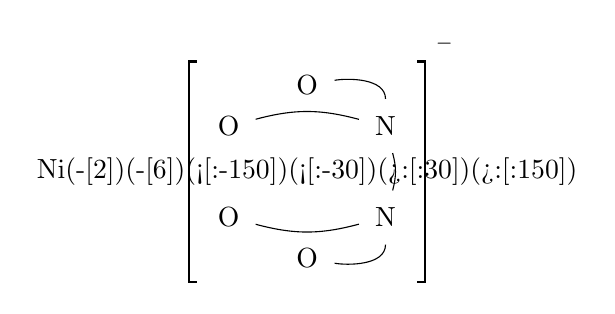
\begin{tikzpicture}
                \node{\chemfig{Ni(-[2])(-[6])(<[:-150])(<[:-30])(>:[:30])(>:[:150])}};
                \node (O1) [circle] at (90:1.1) {\ce{O}};
                \node (O2) [circle] at (-90:1.1) {\ce{O}};
                \node (O3) [circle] at (-150:1.15) {\ce{O}};
                \node (N4) [circle] at (-30:1.15) {\ce{N}};
                \node (N5) [circle] at (30:1.15) {\ce{N}};
                \node (O6) [circle] at (150:1.15) {\ce{O}};
        
                \draw
                    (O3) to[out=-15,in=-165] (N4)
                    to[out=75,in=-75] (N5)
                    to[out=165,in=15] (O6)
                    (O1) to[out=10,in=90,out looseness=0.6] (N5)
                    (O2) to[out=-10,in=-90,out looseness=0.6] (N4)
                ;
        
                \draw [thick] (-1.4,1.4) -- (-1.5,1.4) -- (-1.5,-1.4) -- (-1.4,-1.4);
                \draw [thick] (1.4,1.4) -- (1.5,1.4) node[above right]{\scriptsize$-$} -- (1.5,-1.4) -- (1.4,-1.4);
            \end{tikzpicture}
            \begin{proof}[Answer]
                This molecule is chiral.
            \end{proof}
            \item 
            \begin{tikzpicture}
                \node{
                    \chemleft{[}
                        \chemfig{Co(-[2]NH_3)(-[6]NH_3)(>:[:150]H_3N)(<[:-150]H_3N)(<[:-30]\chembelow{N}{\hspace{1.5mm}H_2}?)(>:[:30]\chemabove{N}{\hspace{1.5mm}H_2}-[:-37,2]CH_2-[2]C?[,,bond]H_2)}
                    \chemright{]^{3+}}
                };
            \end{tikzpicture}
            \begin{proof}[Answer]
                This molecule is achiral (if we assume that the ring on the right side largely lies in the plane with quickly reversing buckling or puckering, a reasonable hypothesis given the light \ce{N} and \ce{C} atoms). It is chiral if we assume a rigid ring in the pictured conformation.
            \end{proof}
            \item 
            \begin{tikzpicture}
                \node{
                    \chemleft{[}
                        \chemfig{Co(-[2]N?[a])(-[6]N?[b])(>:[:150]N>[:30,0.5]C-[2,0.5]C?[a,4])(<[:-150]N-[6,0.5]C<[:30,0.5]C?[b,4])(<[:-30]Cl)(>:[:30]Cl)}
                    \chemright{]^+}
                };
            \end{tikzpicture}
            \begin{proof}[Answer]
                This molecule is chiral.
            \end{proof}
        \end{enumerate}
        \newpage
        \setcounter{enumii}{22}
        \item When \emph{cis}-\ce{OsO2F4} is dissolved in \ce{SbF5}, the cation \ce{OsO2F3+} is formed. The \ce{^{19}F} NMR spectrum of this cation shows two resonances, a doublet and a triplet having relative intensities of $2:1$. What is the most likely structure of this ion? What is its point group? (See \cite{bib:pset5-923}.)
        \begin{proof}[Answer]
            From Bent's rule and sterics, we would predict the following structure, which has point group $\boxed{C_{2v}}$.
            \begin{center}
                \chemleft{[}
                    \chemfig{Os(-[:-75]F)(-F)(-[:75]F)(=[:160]O)(=[:-150]O)}
                \chemright{]^+}
            \end{center}
            Moreover, this structure is supported by the \ce{^{19}F} NMR data, since we have two equivalent (axial) flourines on the same central atom as one nonequivalent fluorine (causing a doublet by the $n+1$ rule of relative intensity 2) and, reversing roles, one (equatorial) flourine on the same central atom as two separate but equivalent fluorines (causing a triplet by the $n+1$ rule of relative intensity 1).
        \end{proof}
    \end{enumerate}
    \newpage
    \item The enthalpies of reaction of trimethylboron with \ce{NH3}, \ce{CH3NH2}, \ce{(CH3)2NH}, and \ce{(CH3)3N} are $-58$, $-74$, $-81$, and $\SI[per-mode=symbol]{-74}{\kilo\joule\per\mole}$, respectively. Why is trimethylamine out of sequence?
    \begin{proof}[Answer]
        Trimethylboron is not a very small lewis acid like \ce{BH3} or \ce{H+}. Thus, its own steric bulk clashes with the considerable bulk of \ce{(CH3)3N}, hindering the reaction in a non-negligible fashion. This hindrance lowers the magnitude of the reaction enthalpy more than the additional electron-donating methyl group can raise it.
    \end{proof}
    \newpage
    \item The complex \ce{UCl4(tmeda)2} (where tmeda is an abbreviation for \ce{Me2N-CH2CH2-NMe2}, which binds by chelation to metals through both \ce{N}-atoms) has been shown by X-ray crystallography to have almost perfect $D_{2d}$ symmetry. Carefully draw a stereochemically accurate picture of this 8-coordinate uranium complex based on what you know about geometrical preferences in 8-coordinate complexes.
    \begin{proof}[Answer]
        The possible molecular geometries for an 8-coordinate species are dodecahedral and square antiprismatic. Assuming all identical, monodentate ligands, the geometries' respective point groups are $D_{2d}$ and $D_{4d}$. Based on this, dodecahedral might look more appealing, but since we have two bidentate chelating ligands, the $D_{4d}$ square anti-prismatic form provides the wiggle room we need for the "descent in symmetry" these ligands will inevitably cause.\par
        As such, if we take a square antiprismatic geometry and place our bidentate ligands opposite each other, we will have constructed the following $D_{2d}$ molecule.
        \begin{center}
            \chemfig{U(-[3]Me_2N?[a])(>:[5]Me_2N?[b])(-[1]NMe_2-[:105,,,1]CH_2-[4]H_2C?[a])(<[7]NMe_2-[:-105,,,1]CH_2-[4]H_2C?[b])(<[:70]Cl)(>:[:110]Cl)(<[:-110]Cl)(>:[:-70]Cl)}
        \end{center}
    \end{proof}
\end{enumerate}




\end{document}